\usetikzlibrary{arrows.meta,positioning}
\begin{frame}{another view}
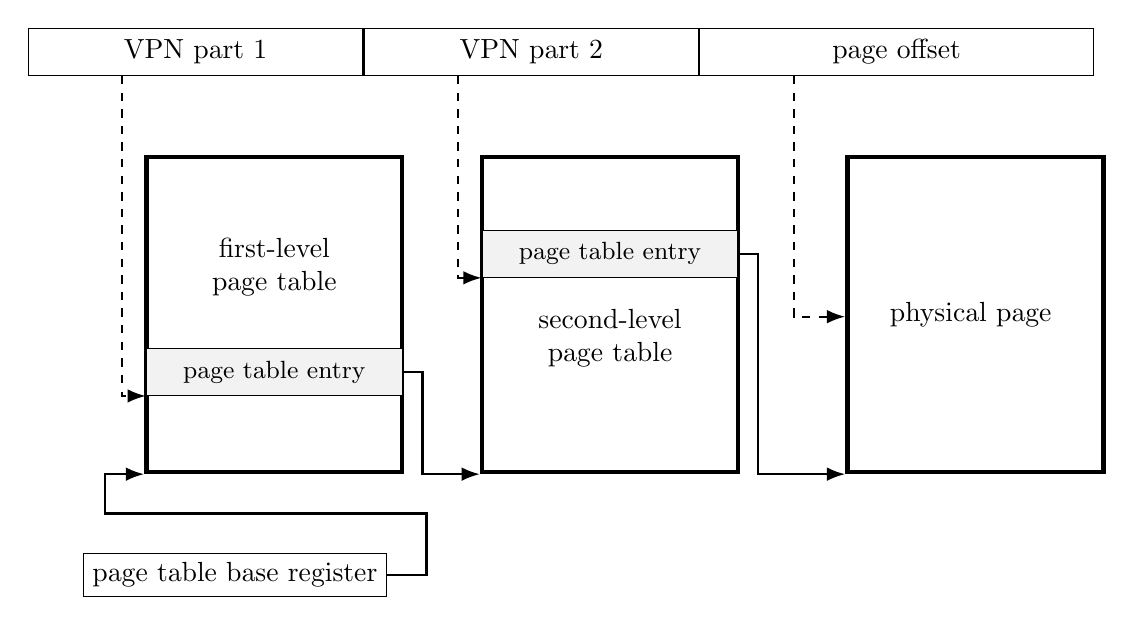
\begin{tikzpicture}
    \tikzset{
        addrPart/.style={draw,minimum height=.6cm},
        pt/.style={draw,ultra thick,minimum height=4cm,minimum width=3.25cm,align=center},
        pte/.style={draw,thin,minimum height=.6cm,minimum width=3.25cm,font=\small,fill=black!5},
        >=Latex,
        compute/.style={thick,->},
        computeB/.style={thick,->,dashed},
    }
    \node[addrPart,minimum width=4.25cm] (vpn1) {VPN part 1};
    \node[addrPart,right=0cm of vpn1,minimum width=4.25cm] (vpn2) {VPN part 2};
    \node[addrPart,right=0cm of vpn2,minimum width=5cm] (po) {page offset};

    \node[pt,below=1cm of vpn1,xshift=1cm] (first) {
        first-level \\
        page table \\
        ~ \\
        ~ \\
    };
    
    \node[draw,below=1cm of first,xshift=-.5cm] (ptbr) {page table base register};
    \draw[compute] (ptbr.east) -- ++(.5cm,0cm) |- ([xshift=-.5cm,yshift=-.5cm]first.south west) |- (first.south west);
    \node[pte] (pte1) at ([yshift=1.3cm]first.south) {page table entry};
    \draw[computeB] ([xshift=1.2cm]vpn1.south west) |- (pte1.south west);

    \node[pt,below=1cm of vpn2,xshift=1cm] (second) {
        ~ \\
        ~ \\
        second-level \\
        page table
    };
    
    \draw[compute] (pte1.east) -- ++(.25cm,0cm) |- (second.south west);
    
    \node[pte] (pte2) at ([yshift=2.8cm]second.south) {page table entry};
    \draw[computeB] ([xshift=1.2cm]vpn2.south west) |- (pte2.south west);
    
    \node[pt,below=1cm of po,xshift=1cm] (final) {
        physical page
    };
    \draw[compute] (pte2.east) -- ++(.25cm,0cm) |- (final.south west);
    \draw[computeB] ([xshift=1.2cm]po.south west) |- ([yshift=2cm]final.south west);
\end{tikzpicture}
\end{frame}
